%!TEX root = ..\MainFile.tex
\section{Адаптация граничных условий течения Куэтта} % (fold)
\label{sec:KuetteAdaptation}
	Как известно, течение Куэтта является простейшим примером системы, в которой вязкие силы играют основную роль в формировании профиля потока. Напомним основные положения в постановке задачи.

	\begin{figure}[h]
	\centering
        \begin{subfigure}{0.45\textwidth}
            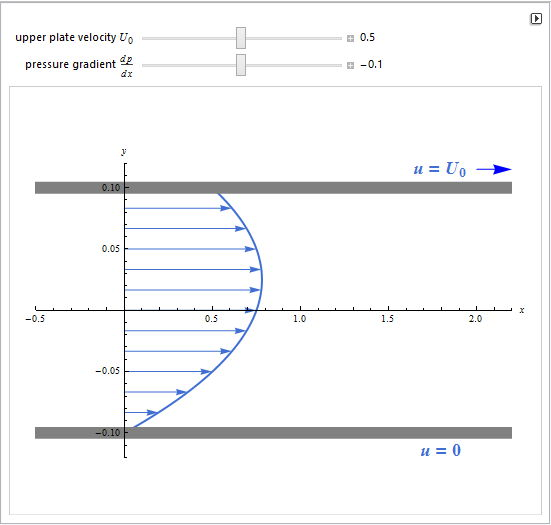
\includegraphics[height=200pt]{Images/KouetteFlowWithPressure}
            \caption{Без градиента давления}
            \label{fig:KuetteFlow:WithoutPressure}
        \end{subfigure}
        \begin{subfigure}{0.45\textwidth}
            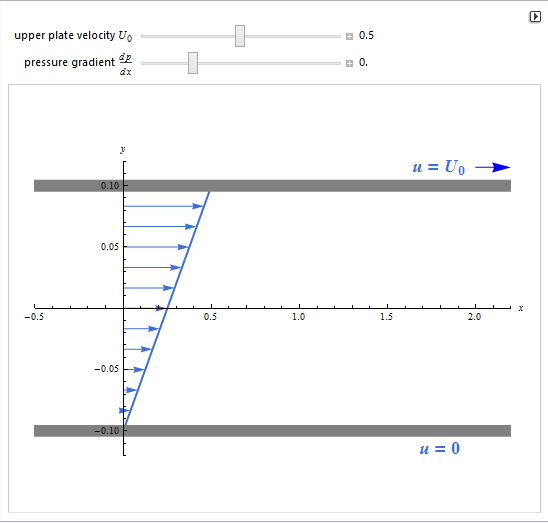
\includegraphics[height=200pt]{Images/KouetteFlowWithoutPressure}
            \caption{С отрицательным градиентом давления}
            \label{fig:KuetteFlow:WithPressure}
        \end{subfigure}
        \caption{Профиль скорости течения Куэтта}
        \label{fig:KuetteFlow}
	\end{figure}

	Как изображено на рисунке \ref{fig:KuetteFlow}, в двумерном течении Куэтта боковые границы удалены на бесконечность (или, что то же самое, реализуют трансляционные граничные условия), нижняя граница неподвижна ($v(0) = 0$), а верхняя движется со скоростью $u_0$: $v(h) = u_0$. В зависимости от наличия или отсутствия градиента давления, профили скорости потока получаются как изображенные на рисс. \ref{fig:KuetteFlow:WithPressure} \ref{fig:KuetteFlow:WithoutPressure} соответственно, и описываются уравнением 
        \begin{equation} \label{eq:CoetteFlow}
            u(y) = u_0 \frac{y}{h} + \frac{1}{2\mu} + (\frac{dp}{dx}(y^2 -hy))
        \end{equation}

	Однако из-за того, что рассматриваемая нами система существенно неравновесна, а частицы обладают собственным моментом движения, применение этих граничных условий при симуляции несколько затруднительно. Во-первых, при прилепливании частиц к верхней или нижней стенке, они очень быстро будут изьяты из потока, и в середине ничего не останется. Во-вторых, даже поставить нулевое значение скорости на нижней границе невозможно в силу того, если  остановить приблизившиеся на радиус взаимодействия частицы, то очень скоро остановятся все частицы, что следует из уравнения \ref{eq:ViksecEquationsOfMotion}.

	\begin{figure}
	\centering
		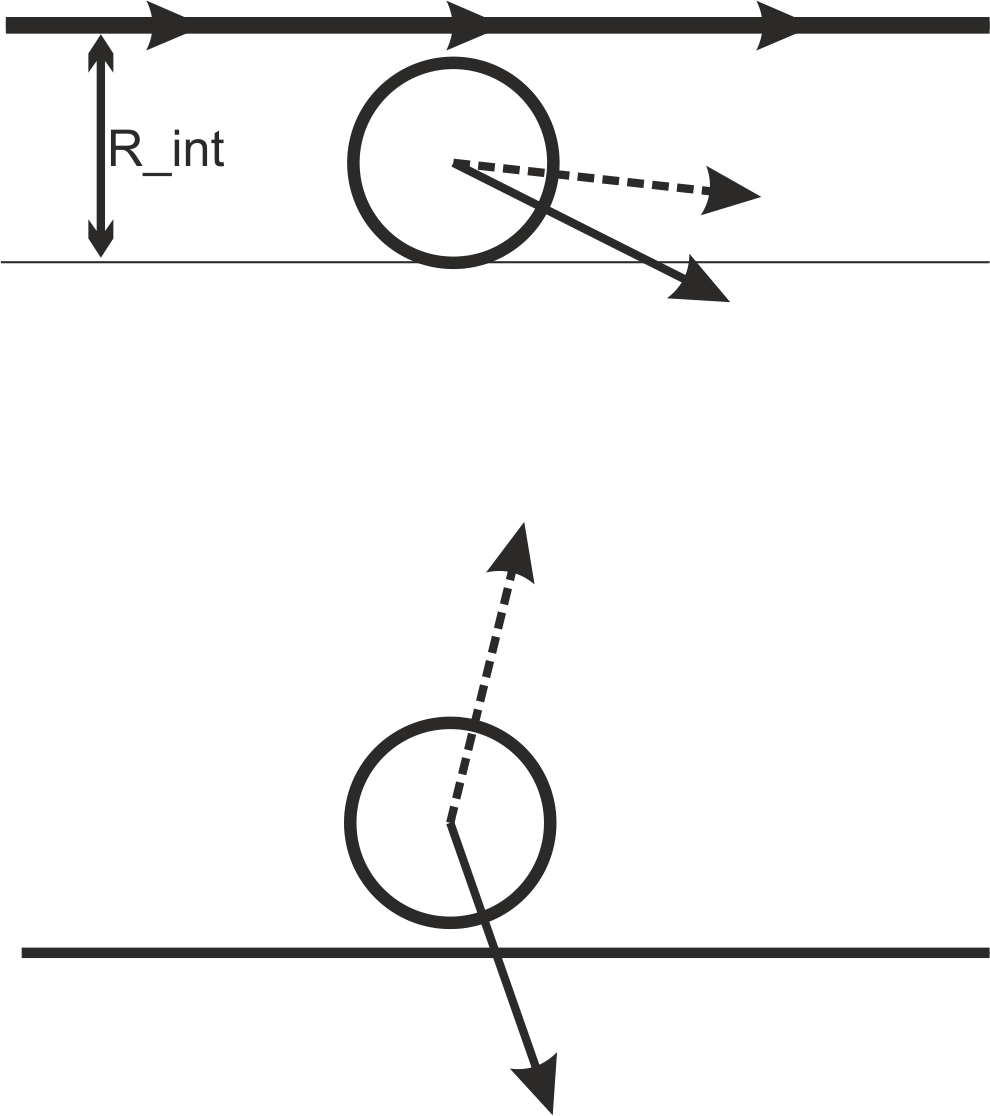
\includegraphics[height=200pt]{Images/BorderInterraction}
        \caption{Граничные условия для адаптированного течения Куэтта}
        \label{fig:AdaptedKuetteFlow}
	\end{figure}

	Потому, нами было предложено два варианта адаптации задачи Куэтта для самодвижущейся жидкости. В обоих из них верхняя граница считается, в некотором роде, непрерывным слоем частиц, движущихся в указанном направлении, и при подхождении частицы на радиус взаимодействия к границе, после взаимодействия этой частицы с остальными частицами, происходит взаимодействие с границей как с еще одной частицей, см. рис. \ref{fig:AdaptedKuetteFlow}.

	На нижней границе в одном варианте адаптации происходит зеркальное отражение частицы, а в другом частица отражается на угол меньший, чем угол падения, что в нашем понимании соответствует ``трению'' с ``шероховатой'' границей. В большинстве симуляций использовался именно первый вариант, подробнее см. в главе \ref{ch:Results}.


% section KuetteAdaptation (end)